% Hamad Medical Corporation
% Georges Younes

\appendix%

%\chapter{Appendix}
%Test for acronyms and nomenclatures

%\gls{usb} $\gls{c}^2$

\chapter{Collision Dectection API}\label{apn:collision_detection_api}

\chapter{RARP Steps}\label{apn:rarp_steps}

\chapter{Evaluation Questionnaire}\label{apn:evaluation_questionnaire}
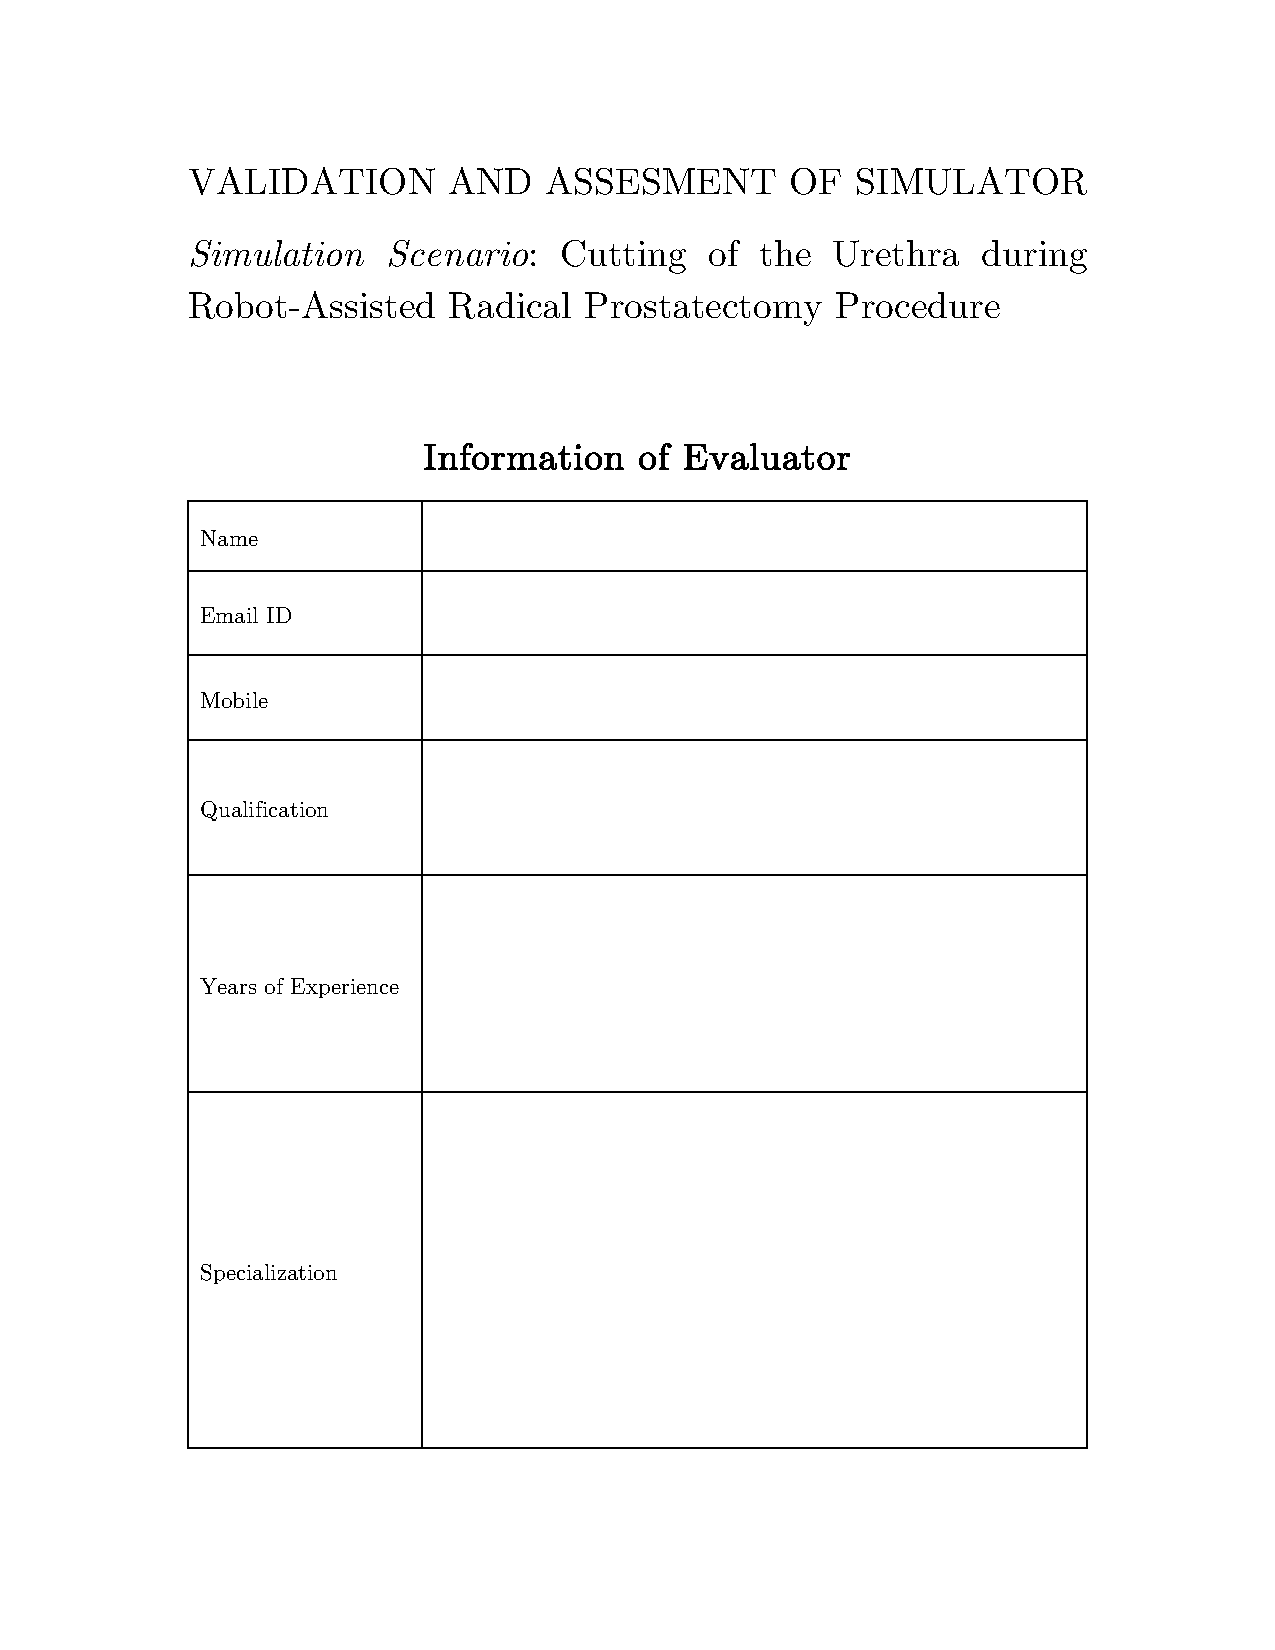
\includepdf[pages=-,scale=0.95,pagecommand={}]{documents/validation/questionnaire.pdf}

%\chapter{Logging of Metrics}\label{apn:logging_metrics}
%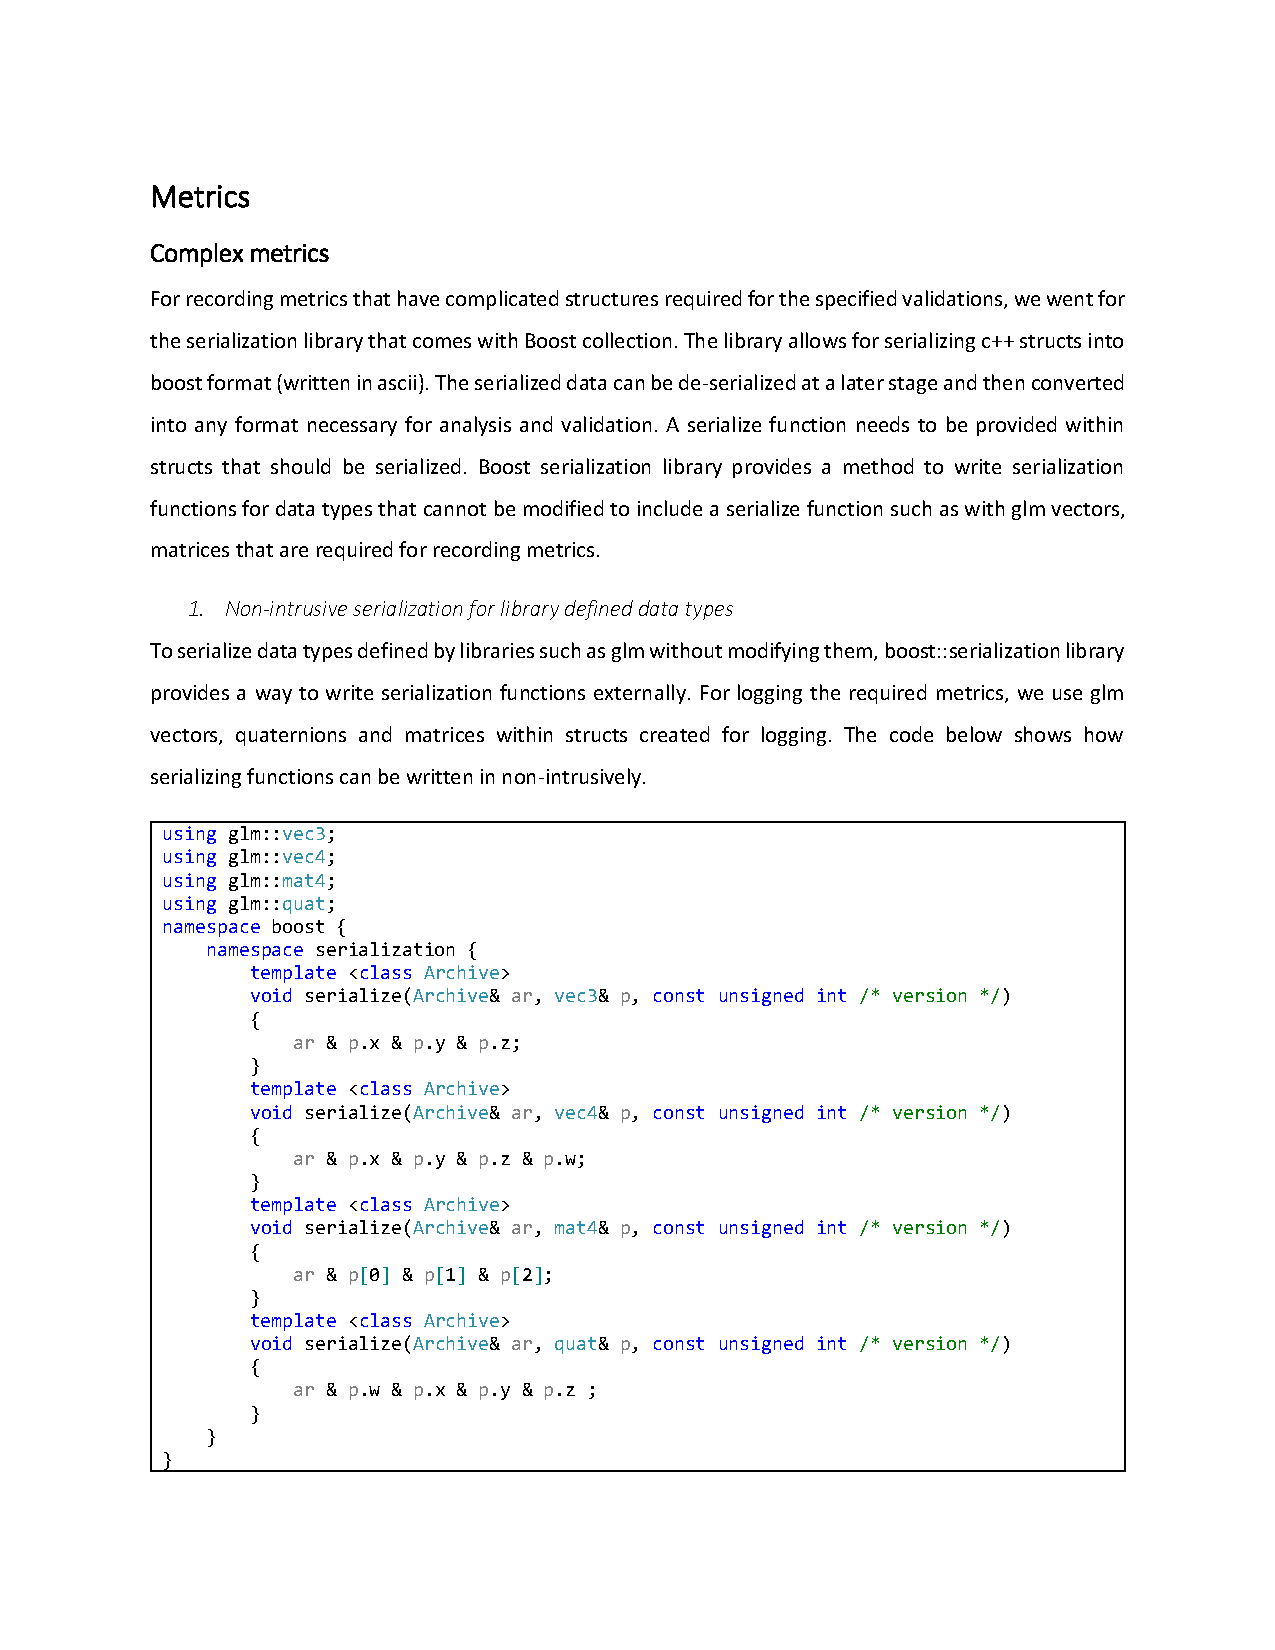
\includepdf[pages=-,scale=0.95,pagecommand={}]{documents/validation/logging.pdf}

%\chapter{Surgeon Responses}\label{apn:surgeon_responses}
%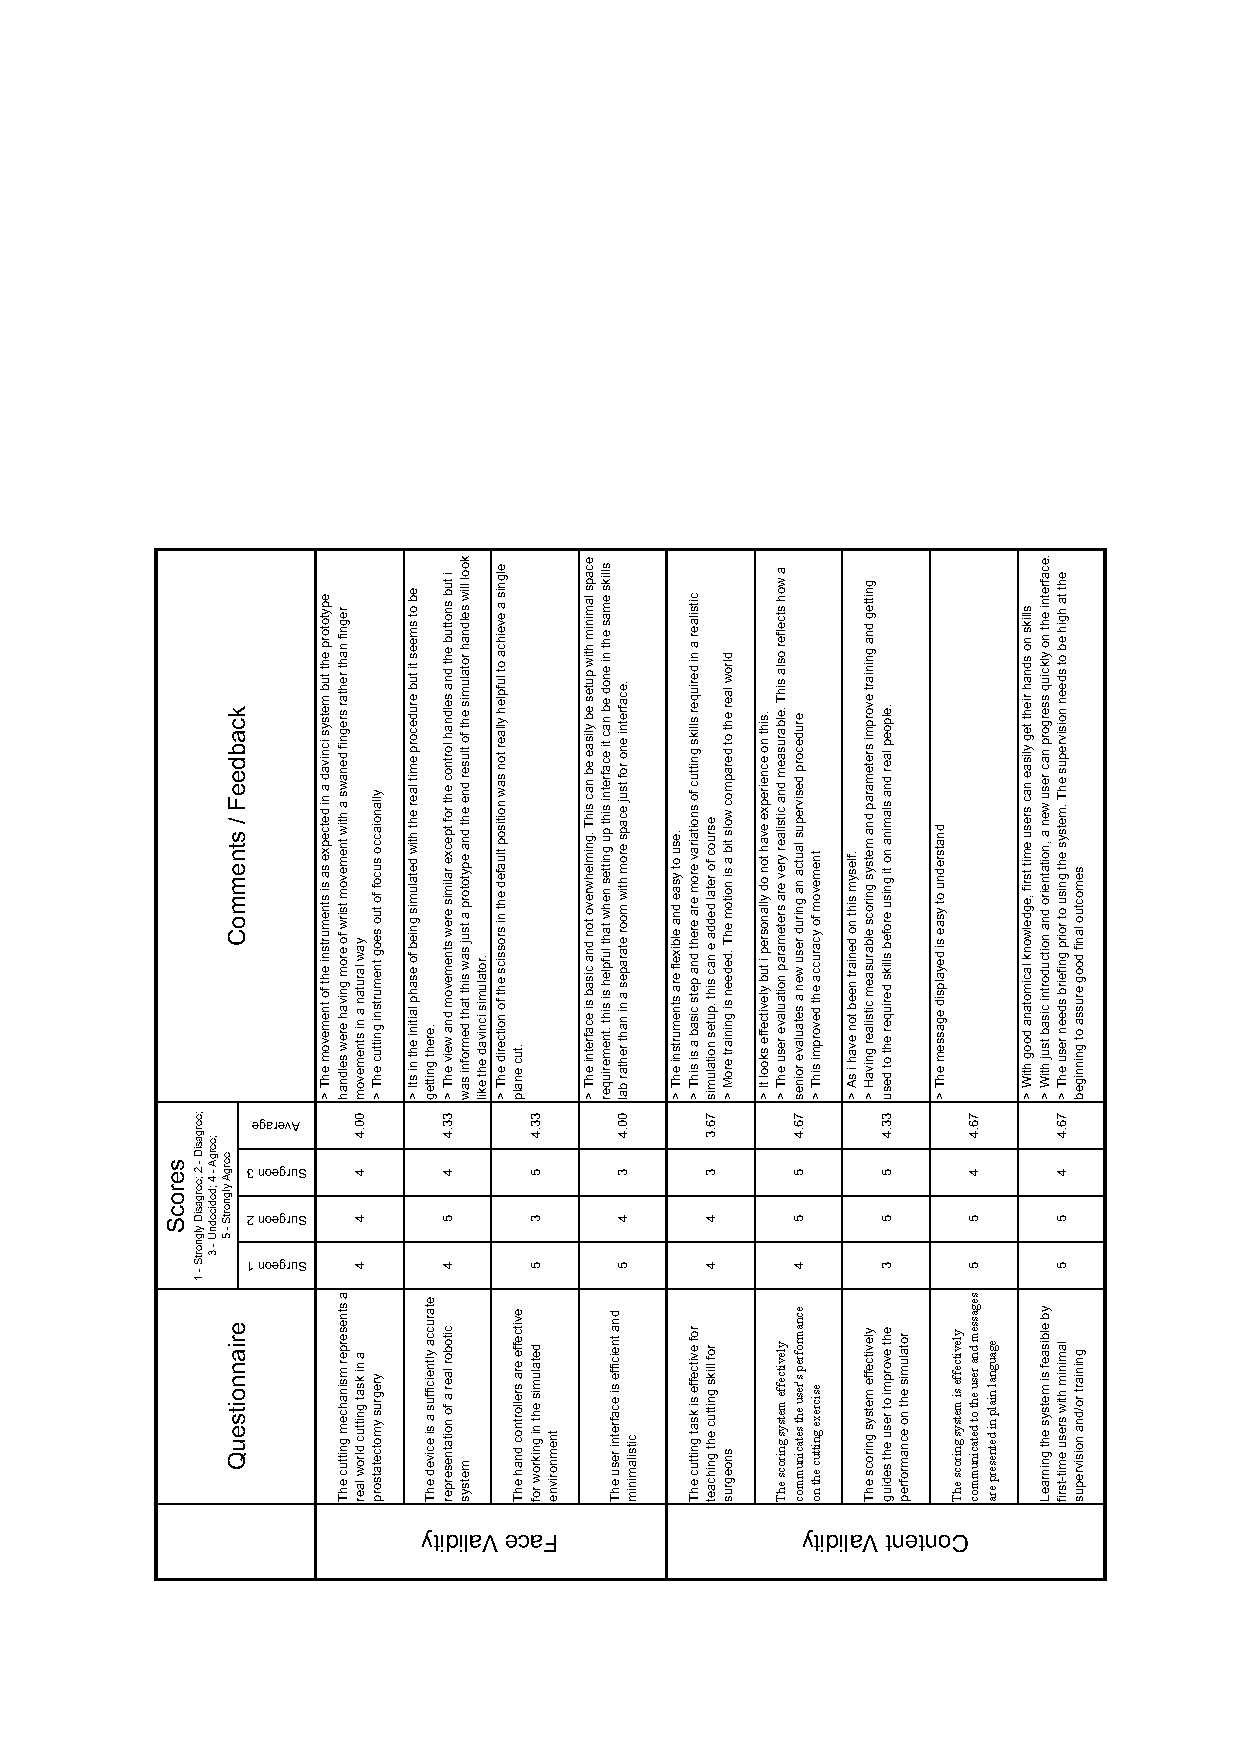
\includepdf[pages=-,scale=1.50,pagecommand={},angle=90,offset=3.5cm 0cm]{documents/validation/surgeon_responses.pdf}

%%% https://stackoverflow.com/questions/2034766/when-using-pdfpages-in-latex-how-to-avoid-page-breaks-before-the-first-page
%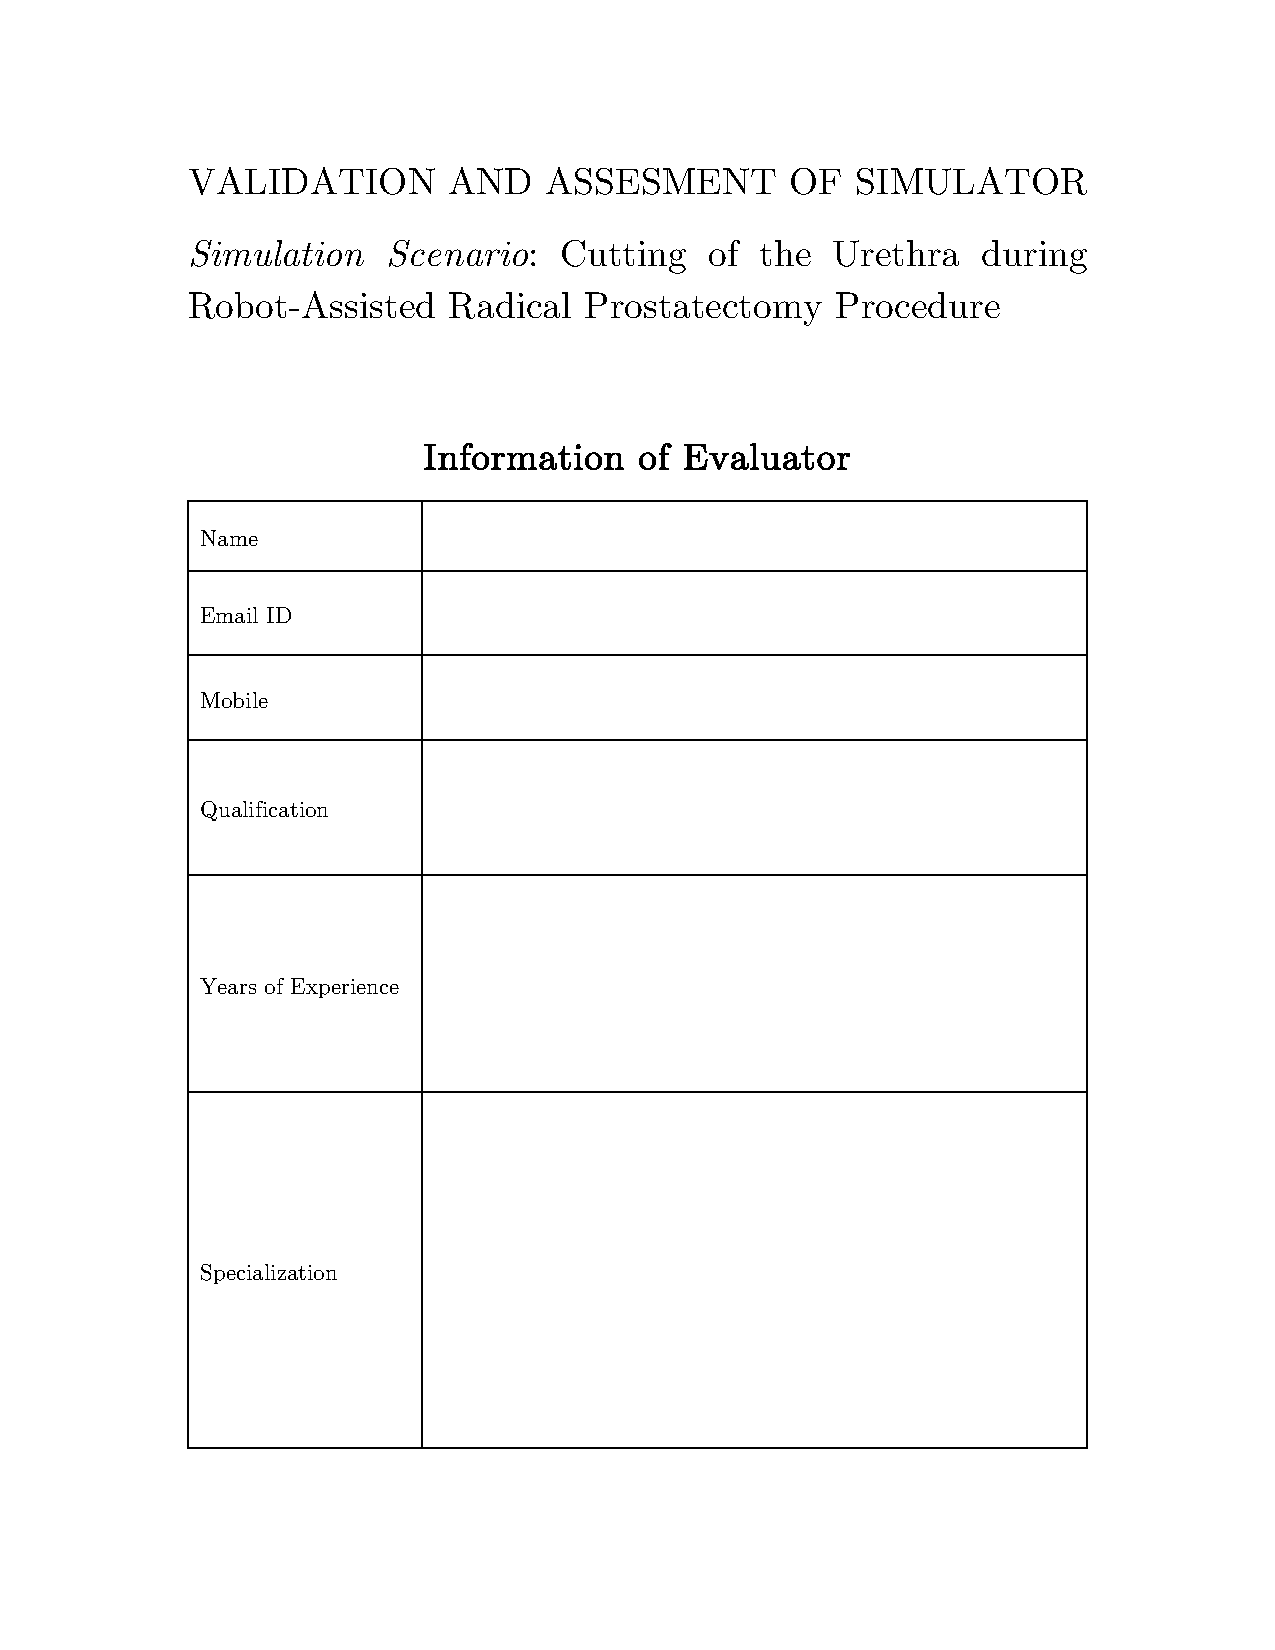
\includepdf[pages=1,pagecommand=\chapter{Evaluation Questionnaire}\label{apn:questionnaire}]{documents/validation/questionnaire.pdf}
%\includepdf[pages=2-,pagecommand={}]{documents/validation/questionnaire.pdf}

\chapter{Publications}\label{apn:publications}
%\section{Journal Articles}
%\printbibliography[heading=none,keyword=scind,subtype=journal]
%\section{Conference Proceedings}
%\printbibliography[heading=none,keyword=scind,subtype=conference]
%\section{Abstracts}
%\printbibliography[heading=none,keyword=scind,subtype=abstract]

\newrefsection
\nocite{*}
\printbibliography[heading=none,keyword=scind,resetnumbers=true]

\chapter{Individual Contribution}\label{apn:individual_contribution}
% https://en.wikibooks.org/wiki/LaTeX/Fonts
\begin{description}[itemsep=1em,font=\fontshape{ui}\selectfont]
  \item [Abdulla AlAnsari \textless\texttt{aalansari1@hamad.qa}\textgreater] has led the team effort inside Qatar. He has supported and guided the overall research, especially the clinical related activities at HMC. He has been actively involved in facilitating activities between different HMC departments. He closely follows-up all project tasks. In particular, he has worked more closely on Aim 5 and 6.
  \\\hrule
  \item [Abdulla Baobeid \textless\texttt{abdulla.baobeid@gmail.com}\textgreater] ---
  \\\hrule
  \item [AbdulRahman AlFayad \textless\texttt{aalfayad@hamad.qa}\textgreater] worked closely on Aim 1, 4 and 6, mainly development for improving the prototype integration, modeling, and validation. He also worked on the Sofa testing and validations in Aim 2 and 4.
  \\\hrule
  \item [Ahammed Waseem Palliyali \textless\texttt{apalliyali1@hamad.qa}\textgreater] worked closely on Aim 1, 4, 5, and 6, mainly development for improving the prototype integration, input handling, modeling, and validation. He also worked on the implementation of evaluation metrics, Looking Glass, and integrating haptic devices. He also worked on development for texture mapping and importing OpenVolumeMesh in SOFA.
  \\\hrule
  \item [Alhusain Abdalla \textless\texttt{aahmed97@hamad.qa}\textgreater] ---
  \\\hrule
  \item [Baljit Singh \textless\texttt{baljit92@gmail.com}\textgreater] ---
  \\\hrule
  \item [Carlos Velasquez \textless\texttt{velcarl@gmail.com}\textgreater] worked on the design of a basic prototype of a wooden console that holds the interfaces for manipulation and visualization so that a surgeon can sit, rest his arms on a padded frontal support while manipulating with both of his hands two haptic devices that actuate virtual instruments within a surgical field rendered to a virtual reality headset.
  \\\hrule
  \item [Dinesh Manocha \textless\texttt{dm@cs.unc.edu}\textgreater] participated in all project meetings, and although he contributes to most project tasks, his work focuses on Aim 3. He is supervising an RA and has worked closely on Aim 1, 3, 4 and 5.
  \\\hrule
  \item [George Turkkiyyah \textless\texttt{gt02@aub.edu.lb}\textgreater] coordinated research activities between AUB and its partners in Qatar. He has led the team effort at AUB, primarily concerned with the development of discontinuous finite element formulations for tissue cutting, and overall development of the project. He is supervising an RA and has contributed in all project tasks, and more specifically on Aim 1, 2, 4, and 5.
  \\\hrule
  \item [Georges Younes \textless\texttt{gyounes@hamad.qa}\textgreater] coordinated the software development, testing, and reporting efforts. He was mainly focused on Aim 1 and 4, all while contributing to all the other aims.
  \\\hrule
  \item [Gorune Ohannessian \textless\texttt{gorune@gmail.com}\textgreater] worked on adding functionality to the geometric cutting module including, in particular, refining communication with the finite element model to send local incremental updates during cutting, and to simplify the model by contracting short edges.
  \\\hrule
  \item [Hawa Hamza \textless\texttt{v-hhamza@hamad.qa}\textgreater] assisted in conducting usability and validation studies of the prototype developed as part of the project. She conducted prior art searches and patent data analyses. She also assisted in drafting the invention disclosure submitted for intellectual property protection.
  \\\hrule
  \item [Jhasketan Phadan \textless\texttt{jpadhan@hamad.qa}\textgreater] worked closely on Aim 4 and 6, mainly preparing software architecture diagrams and integrating physics and graphics middleware libraries. He has also implemented eye and head tracking, created a Windows installer, and was involved in validation.
  \\\hrule
  \item [Julien AbiNahed \textless\texttt{jabinahed@hamad.qa}\textgreater] has been in charge of overall project coordination/management, mainly of the team in Qatar, and ensures that all HMC tasks are met. He coordinated closely with entire team in Qatar and participates in most project tasks. He has worked on all aims.
  \\\hrule
  \item [Liang He \textless\texttt{lianghe.hust@gmail.com}\textgreater] worked closely on Aim 3, mainly algorithms and implementation for continuous collision detection using bounding volume hierarchies.
  \\\hrule
  \item [Mohammed Haddane \textless\texttt{haddane@yahoo.fr}\textgreater] ---
  \\\hrule
  \item [Mohammed Warfa \textless\texttt{mwarfa@hamad.qa}\textgreater] ---
  \\\hrule
  \item [Nicolas AlHaddad \textless\texttt{nicolaselhaddad.nh@gmail.com}\textgreater] ---
  \\\hrule
  \item [Nikhil Navkar \textless\texttt{nnavkar@hamad.qa}\textgreater] co-manages and coordinates technical efforts mainly of team in Qatar and ensures that all HMC tasks are met. Although he contributes on all tasks, he is more focused on Aim 4, 5, and 6.
  \\\hrule
  \item [Samer Itani \textless\texttt{sji03@mail.aub.edu}\textgreater] worked on refining the finite element solver, including a sophisticated constraint management strategy that is more responsive in terms of activation and deactivation especially for shell-type volumetric models. Samer also worked on improving the GPU routines for solution updates.
  \\\hrule
  \item [Santu Paul \textless\texttt{santu.paul@gmail.om}\textgreater] worked on Aim 4 and 6, mainly implementing the rendering of the scene and user interaction in virtual reality. He also assisted during the user validation.
  \\\hrule
  \item [Sarra Kharbech \textless\texttt{skharbech@hamad.qa}\textgreater] led the efforts of validation and usability evaluation of the prototype. She refined the previous validation protocol to evaluate newly-added features, conducted usability studies with subjects, analyzed the results, and inferred conclusions for the team to refine the prototype.
  \\\hrule
  \item [Shaymaa Khalifa \textless\texttt{shfkhalifa@gmail.com}\textgreater] ---
  \\\hrule
  \item [Shidin Balakrishnan \textless\texttt{sbalakrishnan1@hamad.qa}\textgreater] ---
  \\\hrule
  \item [Yasmin Halwani \textless\texttt{yhalwani@qf.org.qa}\textgreater] worked closely on Aim 5 and 6, mainly devising evaluation metrics and protocols for face, content, and construct validity, and conducting interviews.
  \\\hrule
  \item [Zherong Pan \textless\texttt{zherong@cs.unc.edu}\textgreater] worked closely on Aim 3, mainly algorithms and implementation for continuous collision detection using bounding volume hierarchies.
  \\\hrule
\end{description}

\backmatter%
